\documentclass[../uwthesis.tex]{subfiles}
 
\begin{document}
\chapter {Introduction}
 
There are many conflicting theories of dyslexia, a learning disorder that specifically affects reading in 5-17\% of the population and cannot be explained by cognitive, sensory, or circumstantial factors \citep{Shaywitz1998,Snowling2000}. It is broadly (but not universally \citep{Ramus2008,Pennington2012IndividualModels.}) held that dyslexia that dyslexia is characterized by impaired phonological processing, which includes \textit{understanding that speech can be decomposed into phonemes} and \textit{efficiently manipulating, remembering, and accessing phonemic information} \citep{Wagner1987,Snowling1998}. However, it is unclear to what extent the maturation of these skills is a cause or consequence of literacy training or why individuals with dyslexia struggle to master phonological awareness, memory, and automaticity. In a general framework, we might imagine that the first
“disruption” in the phonological processing could occur at one of three stages in the auditory pathway: at the level of extracting relevant information for speech perception from incoming acoustic signals, at the phonemic level (mapping symbols and sounds to discrete phonemes), or at the level of general cognitive processes such as working memory and attention \citep{Serniclaes2004}. This framework is schematized in Figure~\ref{fig:intro_1}

\begin{figure}
    \centering
    \caption{A schematic of several stages at which phonological processing might by disrupted.}
    \label{fig:intro_1}
    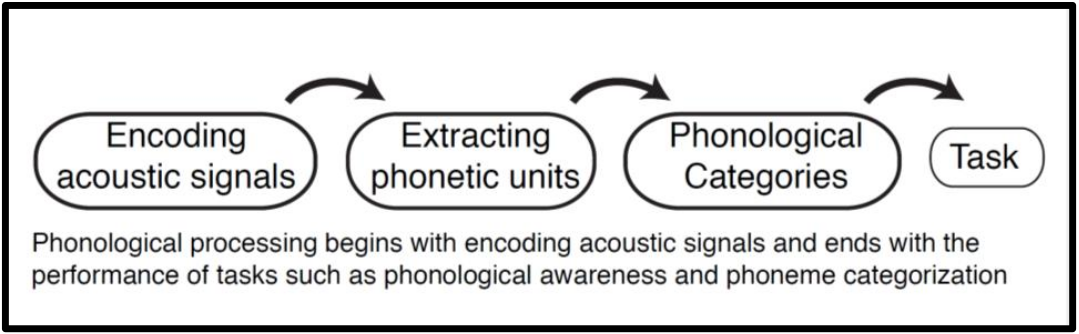
\includegraphics[width=10cm]{images/intro/intro_fig1.png}
\end{figure}
 
In the past decades, several theories have been presented that posit a “core deficit” of dyslexia occurring somewhere in the auditory pathway. Typically, the core deficit is framed as a measurable impairment in some aspect of auditory, linguistic, or cognitive processing that is sufficient to cause dyslexia and accounts for the majority of cases. The purpose of this review is to investigate the evidence supporting the various core deficit theories and to discuss the strengths and weaknesses of these arguments.

It is useful to consider a list of desirable properties that a core deficit model of dyslexia should have:
\begin{itemize}
    \item The deficit must be \textbf{causally related to dyslexia}. An intervention that remedies the deficit in an individual should measurably improve their reading skill.
    \item The deficit must have \textbf{explanatory power as a sensitive and specific mechanism}. In other words, the proposed mechanism should be able to account for the observed impairments in phonological processing, as well as observations from behavioral auditory measures, without simultaneously predicting impairments that individuals with dyslexia do not have.
    \item To be considered a core deficit, the degree of impairment should \textbf{correlate with the degree of reading difficulty}. In other words, in a group of individuals with dyslexia, individuals with the greatest impairment should also have the most disordered reading (in agreement with \citep{Rosen2003}).
    \item \textbf{Most individuals with dyslexia should possess the deficit.} Although clinical populations often yield noisy data, we should expect that any impairment warranting the "core deficit" label is broadly applicable. If a deficit does not occur in most individuals with dyslexia, then it should not be framed as the core deficit of dyslexia.
    \item Most individuals with dyslexia should \textbf{fall outside the normal range observed in individuals with typical reading ability}. For example, if individuals with dyslexia perform worse on a given measure but fall overwhelmingly within the 95\% confidence interval of the non-dyslexic population, then that measure likely does not reflect a deficit that in isolation causes dyslexia \citep{Ramus2003} (assuming the measure is not dominated by noise). Otherwise, any individual with that deficit would have dyslexia. This pattern may indicate a vulnerability that interacts or adds with other factors to influence reading ability (see Figure~\ref{fig:intro_fig2.png}). But a core deficit should not be present in a substantial proportion of the greater population.
\end{itemize}
 
\begin{figure}
    \centering
    \caption{Simulated distributions of a measure in control and dyslexic groups.}
    \label{fig:intro_fig2.png}
    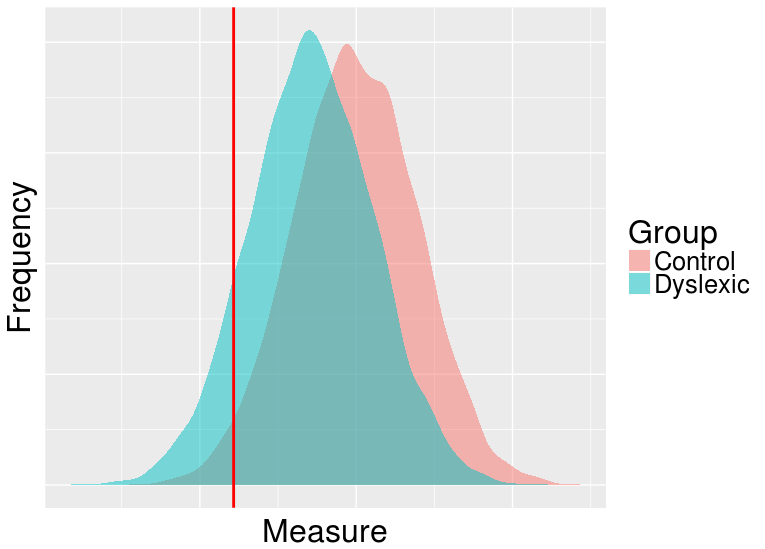
\includegraphics[width=10cm]{images/intro/intro_fig2.png}
    \item \textit{In this example, the
    average value of the measure differs by group, but most measures from the dyslexic group fall within the control distribution. The red line indicates the lower bound of the 95\% confidence interval on the Control group. Above, an effect size of 0.7 is shown (Cohen’s $d$). Assuming the measure is reasonably reliable, this pattern may indicate a risk factor or symptom of dyslexia. However, it would not explain many cases of typical and disordered reading.}
\end{figure}

In practice, some of these criteria may be difficult to meet. For example, because a sample of dyslexics is heterogenous in terms of the remedial treatment participants may have received before the study, and because children are unique population with limited capacity for psychophysics, correlations with any measure in a cohort of young dyslexics may be especially noisy. However, we should aspire to hold a high standard of evidence because of the immense effort and financial resources children, families, and teachers will invest in treatments that may appear backed by science.

We begin with a brief review of several prominent theories of dyslexia. Then, we identify several outstanding questions that this dissertation will address. 

\section{A review of theories of dyslexia}

The field of dyslexia research is more than a century old, and it is not possible to discuss every theory that influences modern thinking about reading disability. The following hypotheses represent some of the most-cited and frequently discussed ideas today. Note that because this dissertation is primarily considered with auditory aspects of reading development, we do not give equal space to predominantly visual mechanisms here. 

\subsection{The rapid temporal processing hypothesis}
In 1980, Paula Tallal demonstrated that dyslexics as a group performed worse on a temporal
order judgment task with short interstimulus intervals (ISIs) but not long ISIs \citep{Tallal1980}. She concluded that temporal auditory processing is a unique challenge for dyslexics. The proposed consequence of this alleged deficit would be in processing “rapid” aspects of speech, included formant transitions and voice onset times. By extension, children would struggle to develop a clear internal model of the sounds of their language, which would hinder their ability to learn the mappings between letters and phonemes. This hypothesis was incredibly influential in driving attention to auditory processing in dyslexics, and the basic tenet—that subtle auditory processing deficits could jeopardize the development of phonological awareness—still proliferates in many of the auditory theories of dyslexia that have followed Tallal’s.

Although this hypothesis has been the subject of immense study and discussion for the last
few decades, a great deal of evidence has been aggregated against the conclusion that rapid temporal processing deficits are at the core of dyslexia (see reviews: \citep{Farmer1995,Rosen2003}). In brief, four separate studies have clarified that Tallal's initial finding can be explained by control participants reaching ceiling performance in one task condition \citep{Reed1989,Nittrouer1999,Marshall2001,Waber2001}, implying that poor readers do not perform as controls even at long ISIs. Furthermore, there is now abundant evidence that individuals with dyslexia perform (on average) poorly on many auditory tasks that do not involve the processing of brief sounds \citep{Hamalainen2013,Rosen2003,Ramus2003,Amitay2002}, including slow ($\sim$ 2 Hz) amplitude and frequency modulation detection \citep{Witton1998,Lorenzi2000,Stuart2006}. Additionally, the intervention program created on the basis of the rapid temporal processing hypothesis, called Fast ForWord, has not shown replicable benefits in randomized control trials conducted by investigators unaffiliated with the product (see \citep{Strong2011AProgram} for review). Clearly, rapid temporal processing is not a specific weakness of children with dyslexia and there is little high-quality evidence that auditory training with brief or temporally modulated stimuli improves their reading skill. 

There are two reasons why the rapid temporal processing hypothesis is still pertinent to today's research. First, it popularized the concept that a subtle perceptual deficit could act as a "roadblock" for children learning to map the sounds of their language to letters. In this view, children with a “fuzzy” percept of formant transitions---such as the cue that
differentiates /ba/ from /da/---might struggle to learn how those ambiguous categories relate to discrete letters. While it is difficult to establish whether this proposed causal pathway is correct, the concept is still frequently referenced in discussions of potential auditory mechanisms of reading disability \citep{Goswami2015SensoryResearch,Calcus2016,Ziegler2009}. 

The second reason is that the rapid temporal processing hypothesis, in some form, is still discussed as a candidate mechanism of dyslexia today. Some researchers claim that rapid temporal processing difficulties occur as the consequence of a more general disruption in neural development (such as entrainment to speech envelope \citep{Goswami2015SensoryResearch} or abnormal noise in cortical neurons \citep{Hancock2017NeuralDyslexia}. Others propose that in spite of the conflicting findings in literature, a temporal processing explanation for dyslexia is still viable \citep{Vandermosten2010,Vandermosten2011}. Some proponents of the magnocellular theory of dyslexia, which hypothesizes that abnormal visual motion processing in the magnocellular pathway is a key feature of the disorder, contend that a similar fundamental mechanism impairs rapid temporal processing in both the auditory and visual domains \citep{Stein2018TheDyslexia,Casini2018ItsDyslexia,Witton2002}. It is unclear whether these renewed theories will be able to answer any of the original criticisms of the rapid temporal processing hypothesis.


\subsection{The temporal sampling hypothesis}
A recent flavor of the temporal processing hypothesis is a shift towards features at the syllabic scale, called the "temporal sampling hypothesis" \citep{Goswami2011}. This is a relatively recent hypothesis inspired by the temporal sampling framework of audition posed by Poeppel (Poeppel, 2003; Giraud and Poeppel, 2012). In Poeppel’s model, neural oscillations sample incoming auditory information. Neural oscillations in the 4-10 Hz frequency band (called Theta waves) are thought to be important for coding syllabic information because these endogenous oscillations have been observed to phase lock to syllables in
speech. This process was hypothesized to be disrupted in dyslexics by Goswami \citep{Goswami2011ADyslexia}.

The hypothesis of the temporal sampling framework is that dyslexics abnormally integrate phonetic features with syllabic-rate information, and this somehow leads to irregularly
specified phonemes that are difficult to map to graphemes. The mechanisms of integration across temporal timescales to construct auditory objects are still largely unknown, so the proposed pathway from abnormal entrainment to syllabic-level cues in speech to disordered phonemes remains vague.

The sampling theory predicts in particular that psychophysical measures of rise time processing, as well as amplitude modulation discrimination and detection at low modulation rates, should be impaired in individuals with dyslexia. A recent review of auditory psychophysical studies estimated that experiments involving some aspect of rise time perception were associated with an average effect size of 0.8 \citep{Hamalainen2013}. While this meta-analysis suggests that reliable group differences exist, it also implies that Control and Dyslexic groups would be more than 50\% overlapping in a typical study. Said another way, only a minority of individuals with dyslexia could be considered to have disordered rise time processing relative to the general population: setting a liberal threshold of "disordered processing" at 1 standard deviation below the mean in the Control population, 42.1\% of individuals with dyslexia (and by definition, 15.8\% of individuals without dyslexia) could be considered disordered. Setting a more stringent cutoff at the bottom 5\% of the Control population (or 1.96 standard deviations), only 12.3\% of dyslexia could be considered disordered. Thus, the literature does not appear to support the view that all or even most individuals with dyslexia perform especially poorly on psychophysical experiments intended to target syllable-rate rise time detection. To my knowledge, this criticism has not been made in the literature yet. 

In sum, the temporal sampling theory has led to an intriguing body of work showing
that rise time impairments occur in some dyslexics as measured by a set of psychophysical tasks. Based on estimates from the current literature, this deficit likely affects the minority of dyslexics. There is only weak evidence for dyslexics having difficulty with slow amplitude modulation rates \citep{Amitay2002,Lorenzi2000,Stuart2006,Witton2002} and contradictory evidence from studies of speech in noise processing suggesting slow modulation sensitivity is intact \citep{Ziegler2009,Dole2012,Calcus2016}. Researchers have also raised concerns that the temporal sampling theory fails to predict many of the experimental conditions in which individuals with dyslexia perform like their typically developing peers \citep{Ramus2012}. While this theory continues to attract much discussion and makes relatively strong claims about the centrality of rise-time processing impairments to dyslexia, there is presently little evidence that a consistent profile of auditory processing difficulties occur across disabled readers. 


\subsection{Deficits in speech robustness}
Yet another auditory framework of dyslexia proposes that the core deficit is not auditory sensitivity, but difficulty extracting informative cues from ethological signals due to a lack of robustness to distortion---for example, speech in the presence of noise \citep{Ziegler2009}. This theory is appealing because it purports to explain why group differences in measures of speech perceptino tend to be small: most psychophysics are performed in ideal listening conditions. As such, true impairments may only be detectable in degraded listening conditions.

In the literature so far, effect sizes between 0 and 1 are typical \citep{Messaoud-Galusi2011,Hazan2009,Boets2007,Dole2012,Poelmans2011,Calcus2016,Ziegler2009}; thus the speech robustness hypothesis faces the same challenge as other auditory hypotheses: the majority of individuals with dyslexia appear to perform in the normal range. 

Another challenge to the speech robustness hypothesis comes from its ability to predict individual differences in other aspects of auditory processing. Recently, Calcus et al. \citep{Calcus2016} addressed the question of whether speech in noise perception predicts the ability to categorically label speech sounds among struggling readers. If individuals with dyslexia with speech in noise deficits are particularly unable to extract phonetic information from complex acoustic signals, then these individuals would be expected to have shallower phoneme identification functions. The authors did not find a significant association between categorical labeling and speech in noise perception. In fact, the authors observed that across several different noise conditions, individual performance among disabled readers was highly variable. This observation was not consistent with a uniform mechanism of impairment. Another study by Calcus et al. also found that individual profiles of performance in several noise conditions were inconsistent, seeming to rule out the idea that a general deficit in utilizing degraded acoustic information is universal in dyslexia \citep{Calcus2018}. These experiments have substantially challenged the idea that speech in noise deficits are predictive of reading skill on an individual level, even though there may be reliable group-level differences.

\subsection{Deficits in categorical perception of speech}
A great deal of literature has focused on the "categorical perception deficit" in individuals with dyslexia; in other words, that groups of disabled readers tend to show shallower identification functions on phoneme labeling tasks as well as more variable discrimination functions \citep{Manis1997,Mody1997,Joanisse2000,Blomert2004,Hakvoort2016,Serniclaes2004}. Some researchers theorize that this impairment is the core deficit of dyslexia \citep{Serniclaes2001}, and many other theories of dyslexia emphasize the role of categorical perception in phonological development. For example, to test the hypothesis that individuals with dyslexia are specifically impaired when processing brief dynamic cues in speech, Vandermosten et al. tested categorical labeling of speech tokens containing dynamic and static phonetic cues \citep{Vandermosten2010,Vandermosten2011}. Indeed, most arguments for a low-level acoustic encoding deficit contend that compromised encoding leads to "fuzzy" representations of phonemes in the brain. 

The primary source of evidence that phonemes are “fuzzy” comes from studies of
identification and discrimination task performance. As with many other deficits reviewed so
far, there does seem to be evidence for a reliable group difference between a sample of
dyslexics and a sample of typically developing controls on these measures: the 2015
Noordenbos and Serniclaes meta-analysis of 34 identification and 13 discrimination studies calculated average effect sizes of 0.66 and 0.86 respectively. Although these effect sizes are
clearly meaningful, they imply moderately overlapping distributions of controls and
dyslexics \citep{Noordenbos2015}.

There are several important considerations in interpreting studies of
categorical labeling and discrimination. First, the notion that categorical labeling slope is
closely related to phonological awareness---the ability to identify and segment phonemes in
a word---has been challenged by several recent studies that have failed to find evidence for a
mediating effect of phonological awareness on the relationship between indices of
categorical labeling and reading skill \citep{Hakvoort2016,OBrien2018,Snowling2019LongitudinalDyslexia}. Although further
study is warranted, the close agreement of these results should elicit a deeper look into
the purported relationship between phonological awareness and “categorical perception”.

Second, identification functions are known to change shape throughout development
\citep{Nittrouer1992}. They are likely closely linked to age and cognitive maturation. However,
because they are typically measured in literate adults and children undergoing literacy
training, it is difficult to disentangle the extent to which they are changed by phonological
awareness. Serniclaes has argued that reliable categorical labeling is not a consequence of
reading ability, because a group of French illiterate adults showed mostly normal
performance on a /ba/$\sim$/da/ labeling task \citep{Serniclaes2005}. However, further study into the causal direction of the relationship between categorical labeling and reading skill is warranted. However, the variance explained among struggling readers by their categorical labeling performance is already relatively small; shrinking our estimate of the degree to which categorical labeling limits reading ability may well bring the power of this marker to explain reading skill below clinically relevant levels. Indeed, several authors maintain that categorical labeling and discrimination already explain too little variance to be useful \citep{Rosen2001,Hazan2009,Messaoud-Galusi2011}.

A theoretical question that must be addressed is
whether non-categorical perception is actually harmful to reading acquisition. At the core of
the categorical perception deficit hypothesis is the notion that dyslexics struggle because they are deluged with irrelevant acoustic information, instead of representing sounds in the simpler code of the phonemes of their language \citep{Serniclaes2004}. This is reminiscent of classical arguments about categorical perception that suggest a “downsampling” process is employed by speech-specific neural circuits, converting a rich acoustic signal into phonemes and discarding phonetic information. Although not all discussions of “fuzzy phonemes” in the dyslexia literature make such claims explicitly, they must lead to similar conclusions implicitly if they accept that a categorical perception deficit is a key feature of dyslexia.

Yet, sub-phonemic variability is known to assist, rather than interfere, with lexical acceses in many contexts \citep{McLennan2003,Connine2004,Whalen1991,Marslen-Wilson1994,McQueen1999,Dahan2001}. Not only are typically developing listeners sensitive to within-category variation of speech sounds, they in fact benefit from such information in the context of word recognition. Furthermore, there is evidence that typical listeners likely do not categorize phonemes in the process of recognizing words, but instead maintain probabilistic representations of several candidate phonemes on the basis of incoming phonetic information \citep{Andruski1994,McMurray2009}. While it is often treated as axiomatic in dyslexia research, the notion that typical listeners rely on a primarily phonemic code during ethological listening conditions is not a consensus among speech scientists \citep{Cleary2001,Port2005,Port2007}.

It will be a challenge for future dyslexia research to discern how categorical labeling of phonemes in an experimental setting relates to phonological awareness and reading skill at an individual level. Currently, it is clear that less categorical labeling of phonemes and reduced phonological awareness are associated with dyslexia, but not that these two impairments always co-occur or can predict reading skill at an individual level. Researchers may have to move away from the view that speech is a string of phonemes to be decoded to better explain the complexity of findings in disabled readers.

\subsection{The statistical learning hypothesis}
Several theories of deficits that are not specifically auditory or linguistic in nature
have emerged in response to the inconsistent evidence for “lower-level” processing
disorders. In this framework, sensory processing is intact and phonemes are represented normally in the brains of individuals with dyslexia, but cognitive processes such as working memory and attention are disordered. 

The statistical learning (or anchoring) hypothesis, first posed by Ahissar \citep{Ahissar2006,Ahissar2007}, posits that individuals with dyslexia fail to benefit from stimulus repetitions, whereas typically developing individuals are able to form "perceptual anchors" around repeated stimuli. This mechanism was suggested following a comprehensive study in which disabled readers participated in a battery of auditory tasks designed to probe low- and high-level auditory mechanisms \citep{Ahissar2007}.

A strength of the anchoring hypothesis is that it offers an appealing explanation for
the oft-repeated result that individuals with dyslexia are more likely to perform abnormally on auditory psychophysical tasks, but do not have consistent profiles of impairment. For example, in the speech in noise literature, Dyslexic groups were more likely to do poorly on speech-in-noise tasks, but few individuals performed consistently poorly when presented with a battery of such tasks \citep{Calcus2016,Calcus2018}. Whether or not the specific mechanism of perceptual anchoring can explain such findings remains to be decided.

There has been immense interest in whether individuals with dyslexia have general difficulties with statistical learning (i.e., taking advantage of the statistics of their environment).
Recent studies have shown that individuals with dyslexia, on average, appear to have some
difficulties with statistical learning in multiple contexts: learning the statistics of noise \citep{Agus2013}, transitional probabilities in streams of
syllables and pure tones \citep{Jaffe-Dax2016}, and novel probabilistic categories \citep{Gabay2015}. However, there are many studies that fail to find such differences \citep{Gabay2018,Staels2015NoDyslexia,Gould1990DoDeficit,Inacio2018ImplicitChildren,Jimenez-Fernandez2011DyslexicCueing,Samara2017ArtificialLearning,Du2013ImplicitInformation}.  The authors of a 2018 study about category learning \citep{Gabay2018} concluded that “the current results underscore that it is too strong to conclude that individuals with
dyslexia have a general impairment in processing probabilistic information.”

Further study is required to determine whether this hypothesis can explain the inconsistent psychophysical literature on dyslexia. Still, it is not clear how the proposed mechanism (statistical learning) will change our understanding of dyslexia as a disorder. This framework has the power to explain why some disabled readers perform poorly on certain psychophysical tasks, but many (and possibly, most) dyslexics do not particularly struggle with these tasks. For example, although anchoring has been proposed to explain deficits in categorical labeling, recall the meta-analysis of 34 phoneme identification studies that predicted an average effect size of 0.66— meaning, only 9.7\% of dyslexics fall below the 95\% confidence interval of the typical population \citep{Noordenbos2015}. Moreover, while proponents of the statistical learning hypothesis argue that the mechanism can explain reduced phonological awareness, there are currently no studies (that I know of) directly assessing the relationship between such measures. 

In conclusion, the statistical learning hypothesis poses a fascinating avenue for new research
into statistical learning in dyslexia that could, with further refinement and exploration,
explain some or most of the perplexing patterns from basic auditory psychophysics. It is not
clear that most individuals with dyslexia have a domain-general statistical learning impairment, and future iterations of this hypothesis will have to be sufficiently nuanced to account for contexts where disabled readers appear to have normal sensitivity to the statistics of acoustic stimuli. At present, it is premature to say whether or not the this hypothesis explains any of the phonological processing difficulties individuals with dyslexia face. However, considering the substantial number of individuals with dyslexia who do not appear to be candidates for a statistical learning deficit, it is questionable whether this is a “core” attribute of dyslexia.

\section{Outline of the dissertation}
This dissertation addresses the role of categorical labeling, sensory processing, and domain-general mechanisms such as attention and statistical learning of speech sounds in literacy acquisition. These questions are of practical significance pertinent to our understanding of reading disorders and their treatment, but are also relevant to theories of speech perception and reading disability in general. 

Four experiments are presented:

\begin{itemize}
    \item \textbf{Clarifying whether individuals with dyslexia are specifically impaired at categorizing speech sounds that differ on the basis of spectrotemporal modulations.}
    This work responds to claims that individuals with dyslexia are impaired at categorizing speech sounds that differ on the basis of a spectrotemporal cue, but not a steady-state cue. 
    \item \textbf{Investigating whether stimulus duration affects how disabled readers categorize speech sounds.} This study examines whether longer exposure to speech cues enables children with dyslexia to behave more categorically on a standard phoneme labeling task. 
    \item \textbf{Characterizing the relationship between sensory, cognitive, and phonological predictors of dyslexia.} This study uses a mathematical model of sensory decision making, the drift diffusion model, to model how children of various reading levels perform on a random dot motion discrimination task. Statistical methods are used to explore the correlational structure of predictors to elucidate the validity of a "core deficit" model of dyslexia. 
    \item \textbf{Investigating the contributions of statistical learning, stimulus adaptation, and fatigue to categorical labeling.} This study is designed to gauge the influence of task features on how disabled and strong readers label phonemes. 
\end{itemize}


\end{document}